
%----------------------------------------------------------------------------------------
%	Horizontal separator line
%   \HRule{2pt}
%----------------------------------------------------------------------------------------
\newcommand{\HRule}[1]{\rule{\linewidth}{#1}} % creo el comando  \HRule regla horizontal



%----------------------------------------------------------------------------------------
%	Horizontal separator line
%   \PRLsep{Text}
%----------------------------------------------------------------------------------------
\newlength{\PRLlen}
\newcommand*\PRLsep[1]{\settowidth{\PRLlen}{#1}\advance\PRLlen by -\textwidth\divide\PRLlen by -2\noindent\makebox[\the\PRLlen]{\resizebox{\the\PRLlen}{1pt}{$\blacktriangleleft$}}\raisebox{-.5ex}{#1}\makebox[\the\PRLlen]{\resizebox{\the\PRLlen}{1pt}{$\blacktriangleright$}}\bigskip}


%----------------------------------------------------------------------------------------
%----------------------------------------------------------------------------------------
%----------------------------------------------------------------------------------------
%----------------------------------------------------------------------------------------
% BOX - TCOLORBOX
%----------------------------------------------------------------------------------------
\usepackage[most]{tcolorbox}
%----------------------------------------------------------------------------------------
% ATTENTION MESSAGE BOX
%----------------------------------------------------------------------------------------
\newtcolorbox{lattention}
{
  breakable,
  enhanced,
  arc      =1mm,
  colback  =gray!5,
  colframe =gray,
  leftrule =12mm,%
  overlay  ={\node[anchor=north west,outer sep=2pt] at (frame.north west) {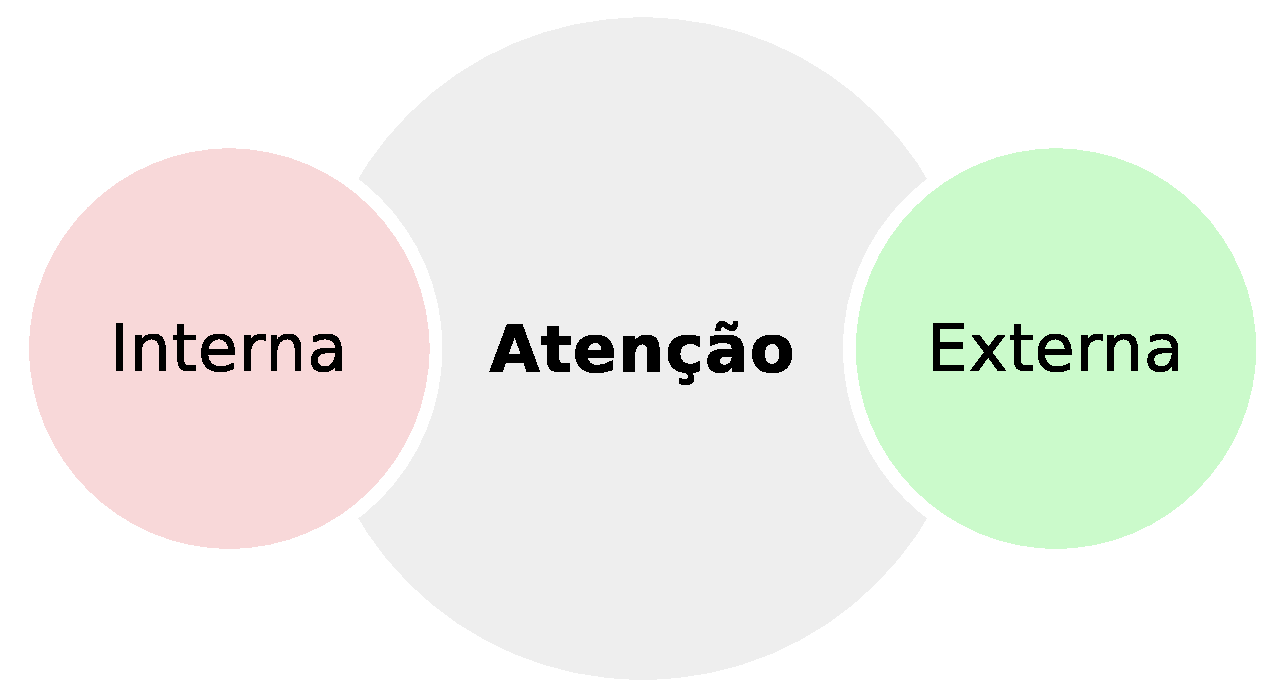
\includegraphics[width=8mm]{attention2.eps}}; }
}

%----------------------------------------------------------------------------------------
% ATTENTION MESSAGE BOX
%----------------------------------------------------------------------------------------
\newtcolorbox{remarcar}
{
  breakable,
  enhanced,
  arc      =1mm,
  colback  =colorsystemdefault!5,
  colframe =colorsystemdefault,
  leftrule =12mm,%
  overlay  ={\node[anchor=north west,outer sep=2pt] at (frame.north west) {
\includegraphics[width=8mm]{remarcar.eps}}; }
}


%----------------------------------------------------------------------------------------
% CITANDO MESSAGE BOX
%----------------------------------------------------------------------------------------
% \begin{citando}
%   texto
% \end{citando}
\newtcolorbox{citando}
{
  breakable,
  enhanced,
  colback  = colorlowgray,
  colframe = colorlowgray,
  arc      = 3mm,
  left skip= 0.10 \linewidth,
  width    = 0.90 \linewidth
}

%----------------------------------------------------------------------------------------
% CATALOGRAFICA MESSAGE BOX
%----------------------------------------------------------------------------------------
% \begin{catalografica}
%   texto
% \end{catalografica}
\newtcolorbox{catalografica}
{
  breakable,
  enhanced,
  colback  = colorlowgray,
  colframe = colorlowgray
}


%----------------------------------------------------------------------------------------
% PATROCINIO MESSAGE BOX
%----------------------------------------------------------------------------------------
% \begin{patrocinio}
%   texto
% \end{patrocinio}
\newtcolorbox{patrocinio}
{
  breakable,
  enhanced,
  colback  = colorlowred,
  colframe = colorlowred
}
